\documentclass[main.tex]{subfiles}
\begin{document}

General Instructions. Read carefully before starting. Solve 5 problems in all; at most 2 questions may be selected from the same section. Candidates registered in the following focus areas must answer two of their five questions from the relevant section as follows:\\

\begin{itemize}
    \item Computer Architecture and High-Performance Computing: Section 1
    \item Communications & Networks: Section 3
    \item Electrical Power & Energy: Section 8
    \item Electromagnetics, Radiation Systems \& Microwave Engineering: Section 4
    \item Electronics, Photonics & MEMS: Section 6
    \item Signal \& Image Processing, Systems \& Controls: Section 3
\end{itemize}

Please write your name and student number below:\\\\

Solve each problem in a \underline{separate} blue book. Write the section number, problem number, and your student number on the front of each blue book. Do not write your name on the blue book. Submit solutions to only five \(5\) problems. Use only one blue book per problem. For each problem, make a special effort to give the answers in a clear form. The exam will begin at 10:00 a.m. and end promptly at 3:00 p.m. Only calculators provided by the department at the examination will be allowed. Personal items including cell phones and other electrical devices must be relinquished prior to the start of the examination. This is a closed book, closed notes examination.

\begin{enumerate}

\subsection{Section 1}

\item After graduating, you are asked to become the lead computer designer at New Computers Inc. You have invented a scheme that reduces the loads and stores normally associated with procedure calls and returns. The first thing you do is run some experiments with and without this optimization. Your experiments use the same state-of-the-art optimizing compiler that will be used with either version of the computer. These experiment reveal the following information:
\begin{itemize}
    \item The clock rate of the un-optimized version is 15\% higher.
    \item 45\% of the instructions in the un-optimized version are loads and stores.
    \item The optimized version executes one-third as many loads and stores as the un-optimized version.
    \item For all other instructions the dynamic execution counts are unchanged.
    \item All instructions (including load and store) take one clock cycle.
\end{itemize}
Which is faster? The optimized version or the un-optimized one. Justify your decision quantitatively by computing an improvement factor to validate your answer.

\item The IEEE 754 Floating point number standard format for single precision floating-point numbers can be summarized as follows. The 32 bits number is divided as shown in figure \ref{fig:f1}. A number is normalized if the exponent value is between 1 and 254, and is denormalized if the exponent value is 0 and the fraction value is not 0. The value of a normalized number is $(-1)^S \times (1+Fraction) \times 2^{(Exponent-bias)}$ and the value of a denormalized number is $(-1)^S \times (0+Fraction) \times 2^{(1-bias)}$. Where the bias value is 127. Please answer the following questions:

\begin{figure}
\centering\fbox{\includegraphics[width=4.0in]{figures/2018s/02a_a.png}}
\caption{32 bits number}
\label{fig:f1}
\end{figure}

\begin{enumerate}
    \item What are the maximum and minimum normalized numbers that can be computed using single precision format?
    \item What are the maximum and minimum denormalized numbers that can be computed using single prevision format?
    \item If we change the Exponent size to be 10 bits instead of 8 and the fraction to be 21 bits instead of 23 bits:
    \begin{enumerate}
        \item What should the bias value be?
        \item Repeat question 2 for the new format.
        \item Repeat question 3 for the new format
    \end{enumerate}
    \item Represent the following two decimal numbers in Single Precsion format:
    \begin{enumerate}
        \item 0.1
        \item 33554431
    \end{enumerate}
    \item Take the values you computed in (d) and convert them back into decimal. Did the numbers change? Explain why.
\end{enumerate}

\item For a hypothetical CPU which has 64 bit virtual address and 41 bit physical address with two levels of cache. The L1 cache is virtually indexed and physically tagged. The L1 size is 8KB. The page size is 8KB. The L2 cache is 4MB. The block size is 64 bytes. Please illustrate the translation of virtual address to physical address, as well as the interactions to the TLB and L1/L2 Cache. Indicate how many bits are used for page number, page offset, TLB index, TLB tag, cache index, cache tag, etc.

\subsection{Section 2}

\item Given \textbf{A} =
    \begin{bmatrix} 
	1 & 2 & 3 & 4 \\
	-1 & 1 & 3 & 2\\
	2 & 2 & 2 & 4 \\
	\end{bmatrix},
	\textbf{y\textsubscript{1}} =
	\begin{bmatrix} 
	2\\
	-2\\
	4\\
	\end{bmatrix},
	\textbf{y\textsubscript{2}} = 
	\begin{bmatrix} 
	1\\
	1\\
	1\\
	\end{bmatrix}

    \begin{enumerate}
        \item Find a basis for the range space of \textbf{A}, R(\textbf{A})
        \item Find a basis for the null space \textbf{A}, N(\textbf{A})
        \item Find the rank and nullity of \textbf{A}
        \item For the equation \textbf{y\textsubscript{1}} = \textbf{A}\textbf{x\textsubscript{1}}, where \textbf{x\textsubscript{1}} is a $4\times1$ vector, does a solution exist for \textbf{x\textsubscript{1}}?
        \item For the equation \textbf{y\textsubscript{2}} = \textbf{A}\textbf{x\textsubscript{2}}, where \textbf{x\textsubscript{2}} is a $4\times1$ vector, does a solution exist for \textbf{x\textsubscript{2}}?
        \item If a solution \textbf{x\textsubscript{1}} and/or \textbf{x\textsubscript{2}} exist in parts (d) and (e), find \underline{all} solutions.
    \end{enumerate}

\item For the system \textbf{A} =
    \begin{bmatrix} 
	-1 & 8\\
	0.5 & -1\\
	\end{bmatrix},
	\textbf{b} =
	\begin{bmatrix} 
	1\\
	0.5\\
	\end{bmatrix},
	\textbf{c} = 
	\begin{bmatrix} 
	-1\\
	1\\
	\end{bmatrix}
	
	\begin{enumerate}
	    \item Design a state observer;
	    \item Using the state estimates from part a), find an appropriate state feedback such that the system will have a purely oscillatory response with a natural frequency of oscillation $\omega_n = 2$ radians/second.
	\end{enumerate}
	
\item Consider a system with a transfer function 
$$\mathrm{G}(s)=\frac{(s-2)(s-5)}{(s+1)(s-3)(s+4)}$$
Is it possible, using \underline{state feedback} to change it to

    \begin{enumerate}
        \item $\mathrm{G}(s)=\frac{(s-5)}{(s+1)(s+4)}$?
        \item $\mathrm{G}(s)=\frac{s-5}{(s+1)(s+3)(s+4)}$?
    \end{enumerate}
    
If yes, do it. Are the resulting systems controllable? observable? If no, explain why not.

\subsection{Section 3}

\item A binary source generates a sequence of symbols with probabilities p and 1-p, respectively. Given the first symbol in the sequence, the source continues to generate symbols until the opposite symbol is generated. Let X denote the length of the sequence, including the first symbol.

    \begin{enumerate}
        \item Find the probability mass function of X.
        \item Find the expected value of X.
    \end{enumerate}
    
\item Messages arriving at a central office switch are exponentially distributed in length, with average length 800 bits and average arrival rate of 16 messages per second. The switch has an infinite buffer and is served by a 64 kilobit per second transmission circuit.

    \begin{enumerate}
        \item Determine the traffic intensity for the switch in Erlangs.
        \item Determine the probability distribution of the number of messages in the buffer.
        \item Determine the average waiting time of a message in the buffer in seconds.
        \item Determine the total average time a message spends in the system, including the waiting time and the service time.
    \end{enumerate}

\item Let $\{\mathrm{Xn}: \mathrm{n}=1,2 \ldots\}$ be an infinite sequence of independent binary random variables with sample values \{0,1) and P\{X n=0\} = 2/3. Let $\text{Yn}=\sum_{\text{i=1}}^{\text{n}} \text{Xi}$ be a random process defined by Xn.

    \begin{enumerate}
        \item For n=5, determine all sample functions of the random process.
        \item Determine the probability mass function of Yn.
        \item Find the expected value and variance of Yn.
        \item Find the autocorrelation function of Yn, $\mathrm{R}\{\mathrm{Y}(\mathrm{n}, \mathrm{n}+\mathrm{k})\}=\mathrm{E}\{\mathrm{Yn} \mathrm{Yn}+\mathrm{k}\}$
    \end{enumerate}
    
\subsection{Section 4}

\item The magnetic field of a particular mode in a parallel-plate air waveguide with a plate separation of 2.5 cm is given by
$$H_{z}(x, y)=C e^{-j 640 \pi x / 3} \cos (160 \pi y)$$
where x and y are both in meters.
    
    \begin{enumerate}
        \item Is this a TE\textsubscript{n} or TM\textsubscript{n} mode? What is n? Is it a propagating or non-propagating mode?
        \item What is the operating frequency?
        \item Find the corresponding electric field.
    \end{enumerate}
    
\item An electromagnetic field in free space, $\mu_{0}=4 \pi \times 10^{-7}$ henry/meter, $\varepsilon_0 = 8.85 \times 10^{-12}$ farads/meter, is specified as by the vector phasor 

$$\underline{E}(\underline{r})=\underline{E}_{0} \varepsilon^{-j \underline{k} \underline{g} \underline{r}}$$

where $\underline{E}_{0}=\hat{x}$ the unit vector in the x direction of a rectangular coordinate system (x,y,z).

$$\begin{aligned}
&\underline{r}=x \hat{x}+y \hat{y}+z \hat{z} \\
&\underline{k}=-j \hat{y}+2 \hat{z}
\end{aligned}$$

    \begin{enumerate}
        \item What is the frequency f of the electromagnetic field (Hz)?
        \item Describe the equi-phase surfaces of the field. Write a general equation for the equi-phase surfaces.
        \item Describe the constant magnitude-of-field surfaces. Write a general equation for these equal-magnitude surfaces.
        \item Evaluate the average power as a function of position.
    \end{enumerate}

\item A plane wave is incident in the interface between two dielectrics $\varepsilon_1$ and $\varepsilon_2$, $\varepsilon_1 > \varepsilon_2$ as shown in figure \ref{fig:12q_a}.

\begin{figure}
\centering\fbox{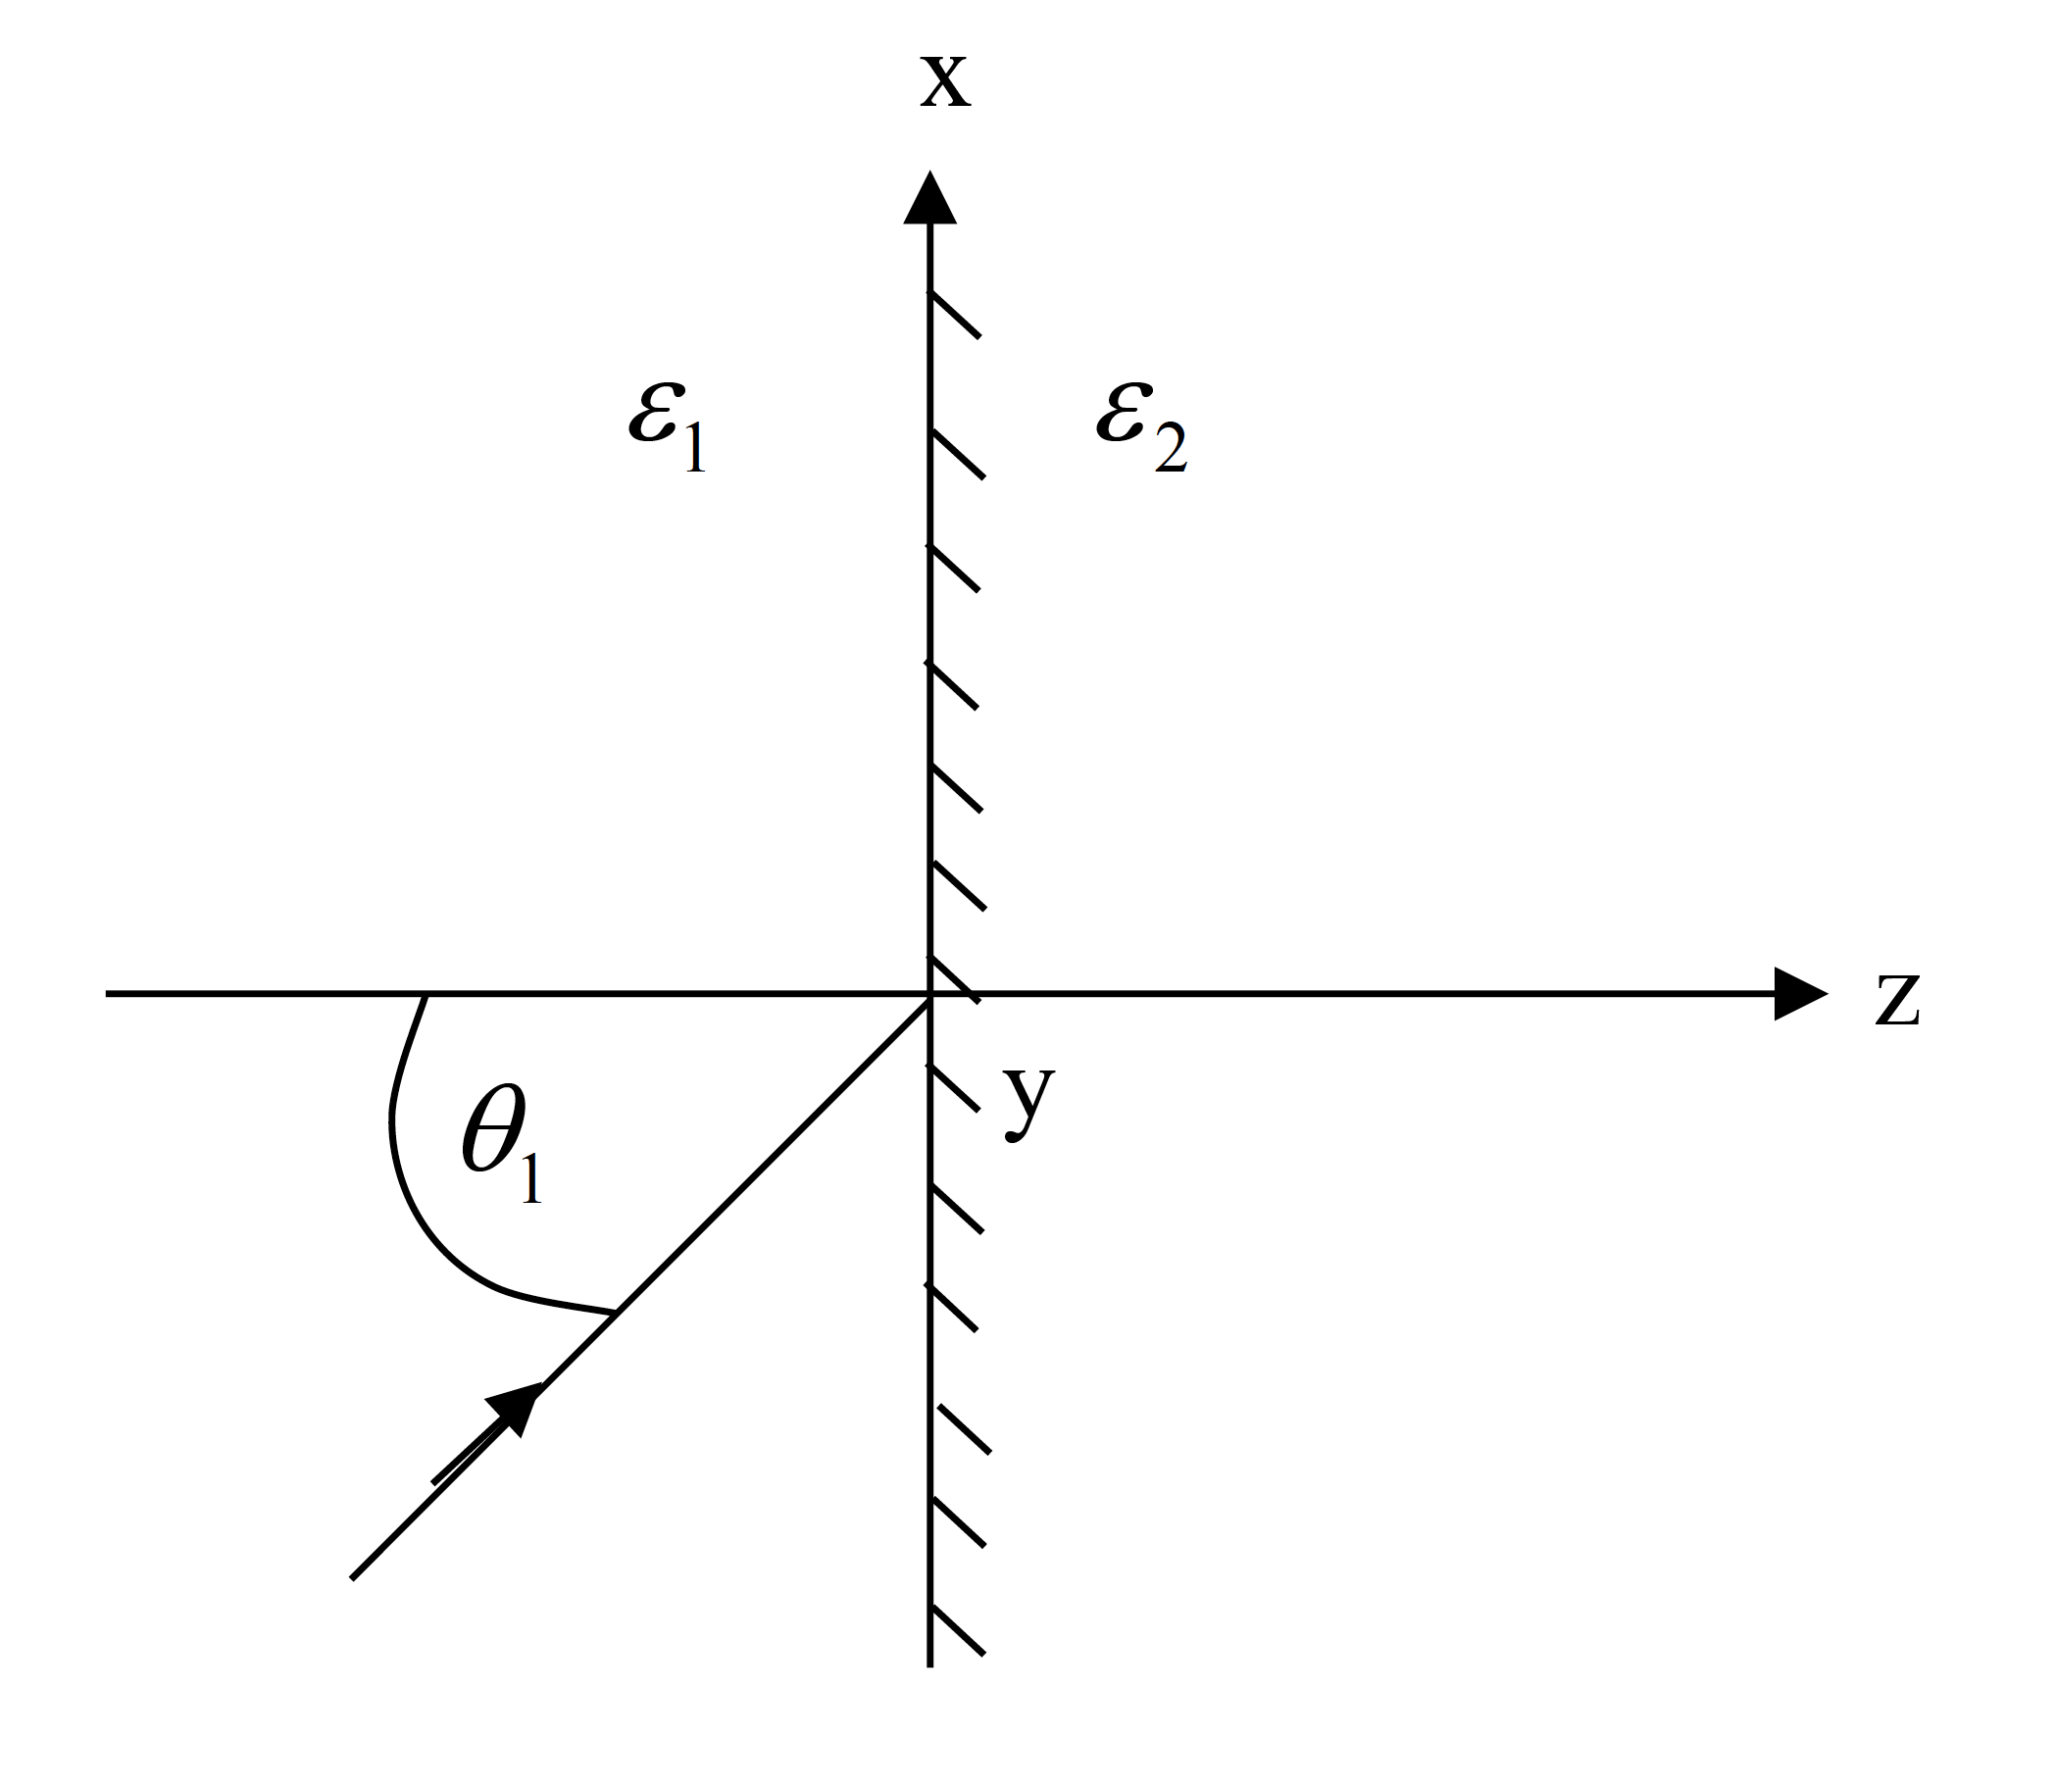
\includegraphics[width=2.0in]{figures/2018s/12q_a.png}}
\caption{Plane wave incident incident in the interface between two dielectrics}
\label{fig:12q_a}
\end{figure}

    \begin{enumerate}
        \item Find the angle $\theta_{1c}$ such that all waves incident with $\theta_1 > \theta_{1c}$ are "totally reflected".
        \item For $\theta_1 > \theta_{1c}$, describe the field (if any) in the region $z > 0$ in the $\varepsilon_2$ dielectric.
        \item If \underline{$E$} is perpendicular to the plane of the incidence, $\underline{E} = E_y \hat{y}$, find the phase of the reflection coefficient.
    \end{enumerate}

\subsection{Section 5} 


	
\end{enumerate}
\end{document}